This section shows an application of the logistic and the scaled logit models to the H3N2 subset of the data from the Ha Nam cohort which is plotted in Figure \ref{HanamCounts}. The Cox model was not used due to absence of reliable data on disease activity.

\begin{figure}[htp]
	\centering
	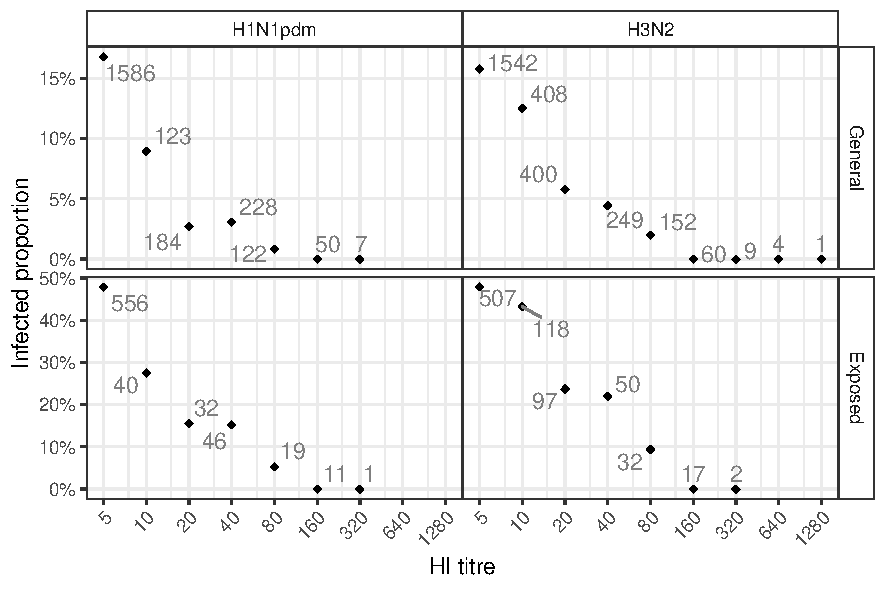
\includegraphics[width=0.9\textwidth]{../data-plot/hanam-hi-summ-light.pdf}
	\caption{
		Ha Nam cohort data. Subjects were grouped by virus and measured HI titre. Numbers next to points are the total number of observations in the corresponding group. The top row is all observations. The bottom row are the observations from households with at least one infection in a given season. The left column is observations for the H1N1pdm virus, the right row --- for H3N2 virus.
	}
	\label{HanamCounts}
\end{figure}
